\section{API-Usability-Verbesserung}
\label{sec:api-research}

Dieser Abschnitt befasst sich --- im Gegensatz zu \sref{sec:api-usability-evaluation} --- nicht mit einzelnen ``Zutaten'' der API-Usability-Evaluation, sondern mit Arbeiten, die konkrete \glslink{api}{API}s analysierten und verbesserten.


\subsection{``Participatory Programming: Developing Programmable Bioinformatics Tools for End-Users'' (Letondal 2006)}
\label{sec:letondal}

Die partizipative Feldstudie von \cite{Letondal:2006dy} ist mit Abstand die spezifischste Veröffentlichung, die ich in meinem Forschungskontext finden konnte, denn sie befasst sich mit Bioinformatikern und reicht in die Bereiche \gls{euse} und API-Usability hinein.

Motiviert wird ihre Arbeit durch die Feststellung, dass die Entwicklung anwenderfreundlicher Bioinformatiksoftware nicht mehr mit der schnellen Forschung im Bereich der Bioinformatik Schritt hält. Neue Hypothesen, Algorithmen und immer größere Datenmengen führen dazu, dass bioinformatische Software ihre Anwender zum Programmieren zwingt.

Biologen und Bioinformatiker, die mit dieser Softwareklasse arbeiten wollen, müssen also programmieren und sind damit Endanwender-Programmierer nach der Definition von \cite{Ko:2011el}.
 
Letondal argumentiert, weshalb existierende Werkzeuge für die neuen Ansprüche der Bioinformatik unzureichend sind.
Werkzeuge, die sich unmittelbar an Endanwender-Programmierer wenden, nutzen häufig domänenspezifische Sprachen (DSL) oder gar Endanwender-Programmierer-Sprachen (EUP). Diese Sprachen sind aber in aller Regel nicht Turing-vollständig, wie das die meisten \textit{General Purpose Languages} (GPL) sind. Turing-Vollständigkeit ist aber notwendig, um mit der schnellen Entwicklung Schritt zu halten.
\\Des Weiteren kritisiert Letondal, dass die Anwender von Bioinformatik-Werkzeugen in deren Entwicklung wenig involviert werden.

Um diese Probleme zu lösen und Bioinformatikern ein adäquates Werkzeug an die Hand zu geben, hat sie im Rahmen ihrer mehrjährigen Arbeit am \textit{Laboratoire d'Informatique Interactive}\footnote{\url{http://lii-enac.fr/en/index.html}} der \textit{École nationale de l'aviation civile}\footnote{\url{http://www.enac.fr/en/}} regelmäßig Interviews, Brainstorming-Sessions und informelle Beobachtungen durchgeführt.

Die Interviews fanden in einem nicht näher spezifizierten Zeitraum statt und wurden teilweise videoaufgezeichnet.

Die Brainstorming-Sessions fanden in den Jahren 1996-2004 mit 5-30 Teilnehmern (vornehmlich Forscher) statt. Die Bioinformatiker wurden also direkt in die Entwicklung dieses Werkzeugs einbezogen.

Letondal stellte fest, dass ihre Probanden immer ihre favorisierten Sprachen (meistens \textit{Perl}) einsetzten, statt eine zu verwenden, die sich für ihre Probleme besser eignet. Sie beobachtete auch, dass ihre Probanden zu einem opportunistischen Arbeitsstil \citep[vgl. ][]{clarke:DSP:2007:1080,Ko:2011el} neigten und das Programmieren nach Möglichkeiten mieden. Des Weiteren fand Letondal heraus, dass Anwender bereits an den einfachsten Aufgaben scheiterten, wenn das Programm keine expliziten oder einfach zu gebrauchende Funktionen dafür bereitstellte. Probanden äußerten an dieser Stelle häufig das Bedürfnis, die Software anpassen zu wollen.

Letondals Arbeit resultierte in dem Werkzeug \textit{biok}, das eine Mischung aus \glslink{ide}{integrierter Entwicklungsumgebung} und Analysewerkzeug darstellt. Anwender dieses Werkzeugs können, abhängig von ihren Fähigkeiten, ausschließlich das Werkzeug nutzen (``programming \textit{with} the user interface) oder es aber erweitern (``programming \textit{in} the user interface''). Besonders an diesem Ansatz ist die Möglichkeit, das Programm aus sich heraus, nämlich mit Hilfe der eingebauten Entwicklungsumgebung, weiterzuentwickeln. Erweiterungen liegen dabei in einem separaten Verzeichnis und können nicht nur Code hinzufügen, sondern auch beliebigen existierenden Code überschreiben\footnote{Das Werkzeug basiert auf \textit{XOtcl} (\url{http://media.wu.ac.at}) und dem \textit{Tk graphical toolkit} (\url{http://www.tcl.tk}). Bei XOtcl handelt es sich um eine Objektorientierungserweiterung für Tcl. XOtcl zeichnet sich durch seine extreme Erweiterbarkeit aus. So können Klassenmethoden zur Laufzeit überschrieben werden, obwohl es bereits Exemplare der Klasse gibt.}. Werden dabei versehentlich kritische Methoden überschrieben und dadurch \textit{biok} funktionsuntüchtig gemacht, können die Erweiterungen einfach wieder entfernt oder verschoben werden.

Letondal bezeichnet diesen Ansatz als \textit{reflektive Architektur} bzw. \textit{reflektive Umgebung}, welche das Kontinuum zwischen Verwendung und Programmierung abdeckt.
%1. functional parameterization, where the parameters may be values or functions, and where the system is composed of functions;
%2. software composition, where the parameterized part includes the scripting to glue software components;
%3. programming, where the user input is the program code, and the system is the programming language.(\citep{Nierstrasz:1995:OSC:232469})
%The third level is thus the most flexible, but too much freedom does not help the end-user, who needs scaffoldings. This is why a fourth level is needed: reflexive architectures, that both provides full programming and explicit structures for parameterization.

Die Gesamtheit aus partizipatorischem Design \citep{Stiemerling:1997:MSS:263552.263646} und Programmierbarkeit des Produkts wird von der Autorin als ``partizipatorische Programmierung'' bezeichnet. Ein ähnliches Konzept wird von \cite{Carroll:1990ex} behandelt und ist unter der Bezeichnung \textit{Programming In The User Interface} bekannt.

Die Arbeit von Letondal ist sicherlich ein Exot. Das Werkzeug wurde nicht nur unter Einbeziehung der späteren Anwender entwickelt, sondern kann sogar durch sie eigenständig weiterentwickelt werden. Leider geht die Autorin nicht darauf ein, inwiefern die API selbst durch ihre Probanden mitgestaltet wurde. Unabhängig davon ist die erfolgreiche Einbeziehung der zukünftigen Anwender in den Entwicklungsprozess einer erweiterbaren Bioinformatikanwendung eine Erwähnung an dieser Stelle wert. 











\subsection{``Methods towards API Usability: A Structural Analysis of Usability Problem Categories'' (Grill u.a. 2012)}
\label{sec:grill}

\cite{Grill:2012jm} haben im Rahmen einer Fallstudie eine API-Evaluationsmethode entwickelt, die meinem im nächsten Kapitel vorgestellten Vorgehen sehr ähnelt. Die vorgeschlagene Methode wurde von den Autoren selbst nur einmal angewendet --- und im Zuge dessen vermutlich verallgemeinert. 

\subsubsection{Methodik}

\cite{Grill:2012jm} vorgeschlagenes Verfahren besteht aus fünf Phasen und kombiniert drei verschiedene Methoden, um ein umfassendes Bild zu generieren. Wie in \fref{fig:grill} dargestellt, finden die Phasen zwei, drei und vier zeitnah statt.

\begin{figure}
  \centering
    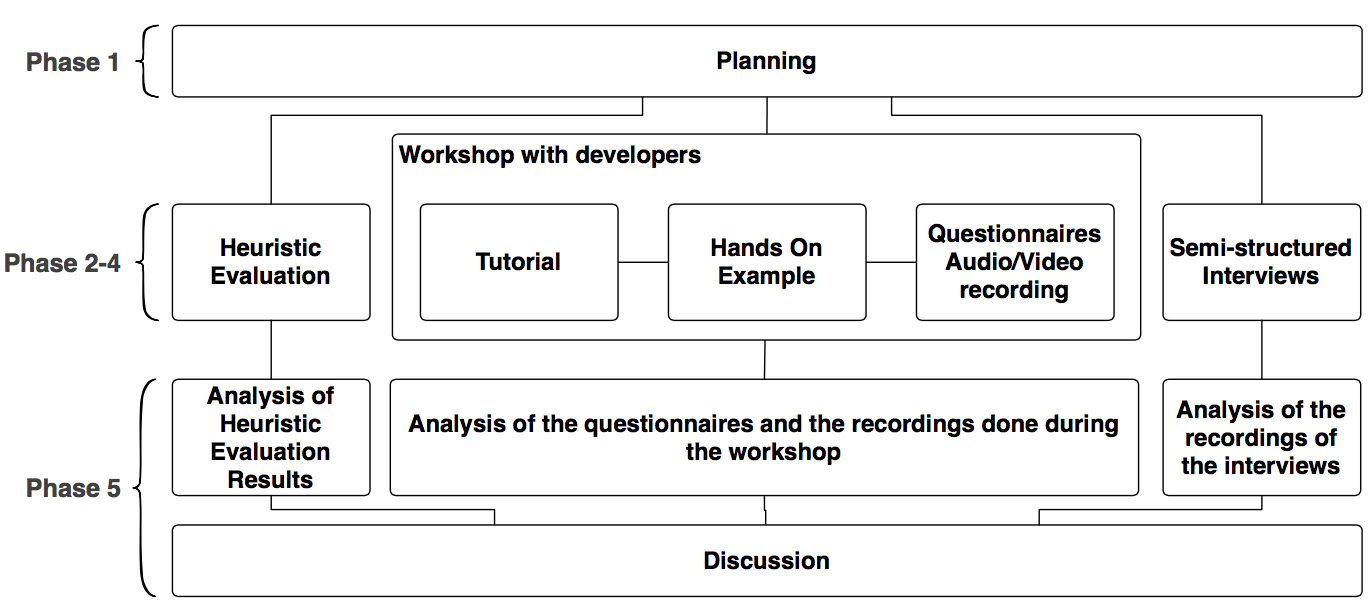
\includegraphics[width=0.9\linewidth]{Figures/grill.png}
    \caption{API-Evaluation nach \cite{Grill:2012jm}}
    \label{fig:grill}
\end{figure}

\begin{description}
  \item[Phase 1: Planung] \hfill \\
  In dieser Phase werden die übrigen vier Phasen vorbereitet. Dazu gehört die Bestimmung und Rekrutierung der notwendigen Experten und Entwickler, die Selektion der zu evaluierenden API-Bereiche und eine Zeitplanung.
  
  Im konkreten Anwendungsfall wurde ein Framework\footnote{\textit{Contextual Interaction Famework}, \url{http://cif.hciunit.org}} evaluiert, das den Entwurf und die Durchführung von Forschungsstudien ermöglicht.
   
  \item[Phase 2: Durchführung --- \gls{he}] \hfill \\
  In dieser Phase wird eine \gls{he} von mehreren geschulten Domänenexperten mit dem Ziel durchgeführt, potentiell problematische API-Bereiche zu finden, damit diese in den weiteren Phasen besondere Beachtung finden.
  
  Die 16 äußerst knapp formulierten Heuristiken wurden von den 16 API-Design-Guidelines von \cite{zibran2008makes} abgeleitet. Zibran stellt in seiner Arbeit die Ergebnisse seiner Literaturforschung im Bereich der API-Usability vor. Beispiele für die Heuristiken sind:
  \begin{itemize}
    \item Benennung: Die Benennung muss selbsterklärend und konsistent sein.
    \item Dokumentation: Eine Dokumentation und Beispiele müssen bereitgestellt sein.
    \item Fabrikmethode (engl. \textit{factory pattern}): Die Fabrikmethode darf nur genutzt werden, wenn es unvermeidbar ist.
  \end{itemize}
  
  Untersuchungsgegenstand sind die API selbst und dessen Dokumentation. Im konkreten Anwendungsfall wurden vier Domänenexperten als Evaluatoren eingesetzt.
   
  \item[Phase 3: Durchführung --- Workshops] \hfill \\
  Workshops sind Veranstaltungen, zu denen API-Anwender eingeladen werden, um die eigentliche Datenerhebung zu ermöglichen. Ein solcher Workshop besteht aus drei Teilen:
  \begin{enumerate}
    \item Einführung in die Anwendungsdomäne
    \item Tutorial in Form einer Präsentation mit einfachem Anwendungsbeispiel
    \item Praxisteil, bei dem sich die Probanden aus einem vorher zusammengestellten Aufgabenkatalog eine Aufgabe zum selbstständigen Lösen heraussuchen können 
  \end{enumerate}
  
  Während eines Workshops verfügt jeder Proband über einen Fragebogen, in dem er auftretende Probleme dokumentieren soll. Der Workshop selbst wird videoaufgezeichnet, um Unstimmigkeiten bei der späteren Analyse klären zu können.
  
  Im konkreten Anwendungsfall nahmen acht männliche Akademiker mit mehrheitlich mehrjähriger Berufserfahrung im Alter von Anfang 30 teil.  
   
  \item[Phase 4: Durchführung --- Teilstrukturierte Interviews] \hfill \\
  Diese Phase findet unmittelbar nach einem Workshop oder spätestens am darauf folgenden Tag statt. Dabei wird mit jedem Probanden ein teilstrukturiertes Interview geführt. Das Interview besteht zum einen aus den in Phase 2 verwendeten Heuristiken und zum anderen auf ähnlich geartete Guidelines von \cite{Bloch:2006jk}, von denen ich ein paar im \sref{sec:forschung-einzelne-ergebnisse} nenne.
  
  Außerdem werden während der Interviews individuelle Probleme besprochen. Die Länge eines solchen Interviews ist auf 30 Minuten beschränkt.
   
  \item[Phase 5: Analyse] \hfill \\
  In dieser Phase werden die Ergebnisse der \gls{he}, die Umfragen und Videoaufzeichnungen der Workshops und die Interviews analysiert.
\end{description}



\subsubsection{Ergebnisse}

\begin{important}
Die Verwendung verschiedener Methoden hat sich ausgezahlt, denn von den 169 ermittelten API-Usability-Problemen waren 157 einzigartig. Das bedeutet, sie wurden nur mit einer der verwendeten Methoden gefunden.

Die \gls{he} hat dabei die meisten Verstöße gegen die Heuristiken \textit{Dokumentation}, \textit{Komplexität}, \textit{Benennung} und \textit{Konsistenz / Konventionen} ermittelt. Die Aufzeichnungen des Workshop-Praxisteils haben hingegen die schwerwiegendsten Probleme hervorgebracht. Mit Hilfe der Interviews konnten die Forscher die meisten Benutzererlebnis-Aspekte wie Attraktivität, Emotionen, etc. ermitteln.

Darüber hinaus schlagen \cite{Grill:2012jm} eine mögliche Klassifikation von API-Usability-Problemen vor:
\begin{enumerate}
\itemsep1pt\parskip0pt\parsep0pt
  \item Dokumentation
  \item Laufzeit (Probleme, die erst bei der Ausführung von Code sichtbar werden)
  \item Struktur
  \item Benutzererlebnis
\end{enumerate}
\end{important}


\subsubsection{Kritik}
\label{sec:grill-kritik}

\begin{important}
Leider sind die Forschungsergebnisse größtenteils quantitativer Natur. Eine intensive qualitative Auseinandersetzung fand nicht statt.

Das vorgeschlagene Verfahren findet in einer Laborumgebung statt, was die Probanden potentiell beeinflusst und die Breite an beobachtbaren API-Usability-Problemen beschränkt. Dieselbe Konsequenz vermute ich beim Einsatz der \gls{he}.

Die Verifizierbarkeit der Ergebnisse wurde gezeigt. Die Verallgemeinerbarkeit hingegen nicht; das Verfahren wurde in keiner mir bekannten weiteren Forschung angewendet. Allerdings ist das Bewusstsein für die Wichtigkeit von API-Usability relativ neu \citep{Robillard:2010bh}.

Die verwendeten Heuristiken sind sehr knapp formuliert. Die Autoren geben keine Auskunft darüber, ob den Evaluatoren ausführlichere Beschreibungen zur Verfügung standen. Außerdem bemühen die Autoren das Argument, dass drei bis fünf Experten genügen, um 60\% der Usability-Probleme zu entdecken \citep{UmerFarooq:2010tt}. Diese Erkenntnis bezieht sich allerdings auf die Heuristiken von \cite{Nielsen:1993vk}. Darüber hinaus wurde in keiner Weise gezeigt, dass die von den Autoren verwendeten Heuristiken vollständig sind.

Die relativ stark quantitative Betrachtung und die Wichtigkeit der Heuristiken schränken die Eignung als Verfahren zur Grundlagenforschung ein.
 
Der personelle Aufwand für dieses Verfahren ist sehr hoch. Dafür erstreckt es sich aber zumindest über einen viel kürzeren Zeitraum, als dies beispielsweise bei der Concept-Maps-Methode \citep{Tenny:2011jp} der Fall ist.
\end{important}






\subsection{``An Empirical Study of API Usability'' (Piccioni u. a. 2013)}
\label{sec:piccioni}

Diese Arbeit hatte die Verbesserung der API der in Eiffel geschriebenen Persistenz-Bibliothek \textit{ABEL}\footnote{\url{https://svn.eiffel.com/eiffelstudio/branches/eth/eve/Src/library/abel/}} zum Ziel. Dabei sollten 25 Probanden mit Hilfe dieser API Probleme lösen. Es handelt sich dabei um die aktuellste Studie, die ich im Bereich der API-Usability-Evaluation finden konnte.

\subsubsection{Methodik}

Methodisch kamen die \glslink{cd}{\textit{kognitiven Dimensionen}} von \cite{Anonymous:9HSMlhmF} (siehe \sref{sec:api-cds}), \textit{Usability-Tokens} und \textit{Interviews} zum Einsatz. Die fünf verwendeten Usability-Tokens \textit{surprise}, \textit{choice}, \textit{missed}, \textit{incorrect} und \textit{unexpected} werden von den Autoren als orthogonal zu den kognitiven Dimensionen beschrieben, spielen für die Ergebnisse der Arbeit aber nur eine untergeordnete Rolle und werden in dieser Wiedergabe nicht weiter betrachtet.

Die 25 Probanden waren Master- und Promotionsstudenten mit wenigstens einem Jahr Programmiererfahrung in Objektorientierung, durchschnittlich einem Jahr Programmiererfahrung in Eiffel und keinerlei Erfahrung im Umgang mit der ABEL-API.

Das Experiment begann mit einer Einweisung in die wichtigsten Funktionen der IDE. Speziell wurde auf die Möglichkeit hingewiesen, die ABEL-Dokumentation in der IDE zu konsultieren. Außerdem wurde gezeigt, wie die Klassenhierarchie inspiziert werden kann.

Im Anschluss mussten die Probanden Programmieraufgaben mit Hilfe der ABEL-API lösen. Die Arbeitsplätze wurden dabei mit Video aufgezeichnet und die Probanden darum gebeten, ihre Gedanken zu verbalisieren (\textit{think aloud}). Für die Programmieraufgaben gab es kein Zeitlimit. Des Weiteren konnten sich die Probanden an einen der Experimentatoren wenden, wenn sie Probleme hatten.

Unmittelbar nach der Programmieraufgabe wurde mit jedem Probanden ein strukturiertes Interview geführt, das insbesondere zur Erhebung der subjektiven Usability diente. Dazu wurden nachträglich relevante Programmierepisoden mit einem oder mehreren Usability-Tokens klassifiziert. Das Interview selbst basierte auf 12 Fragen, die aus den 12 kognitiven Dimensionen abgeleitet wurden.

\subsubsection{Ergebnisse}

\cite{Piccioni:2013uq} schlussfolgerten die folgenden Punkte aus ihren Beobachtungen:
\begin{itemize}
  \item Die Benennung muss akkurat, knapp und selbsterklärend sein, was in Bezug auf eine Anwendungsdomäne bereits Probleme hervorruft. So erwarteten einige Probanden ein anderes Funktionsspektrum beim Lesen des Klassennamens \textit{REPOSITORY} und hätten den Begriff \textit{DATABASE} für treffender gehalten. Bereits in der Informatik sei eine eindeutige Benennung schwierig. So meinen beispielsweise die Begriffe \textit{method} (Java), \textit{routine} (Eiffel) und \textit{member function} (C++) das selbe Konstrukt.
  \item Erkenntnisse in Bezug auf den Gebrauch der Fabrikmethode \citep{Ellis:2007kv} wurden bestätigt. Demnach ist dessen Gebrauch nach Möglichkeit zu vermeiden und unbedingt die Verwendung von Konstruktoren vorzuziehen.
  \item Typen sind konstanten Strings vorzuziehen. 
  \item Die Dokumentation unbedingt muss akkurat, eindeutig und in sich abgeschlossen sein. Diese Erkenntnis wird mit dem folgenden Zitat untermauert: ``bad documentation is a nonstarter''.
  \item Lösungswege müssen eindeutig sein. Verschiedene Lösungsoptionen sollte es nur geben, wenn sie komplementär sind. Dieser Punkt wird auch von \cite{Zibran:2011fx} bestätigt.
\end{itemize}

\subsubsection{Kritik}
\begin{important}
Abgesehen davon, dass der Titel dieser Arbeit in mir höhere Erwartungen geweckt hat, musste ich die folgenden kritischen Beobachtungen machen:
\begin{itemize}
  \item Die Vorgabe einer IDE gefährdet die Verallgemeinerbarkeit der Erkenntnisse, was in der Arbeit nicht diskutiert wurde.
  \item Die damit einhergehende Einweisung in die IDE erlaubt keine Aussagen mehr auf die \gls{oobe} \citep{Kahlert:2011wr}. Die Fokussetzung auf bestimmte IDE-Funktionen wirkt sich potentiell auf die Lösungsstrategien der Probanden aus. Beispiel: Die Experimentatoren haben auf die Möglichkeiten hingewiesen, die API-Dokumentation aus der IDE heraus zu konsultieren. Dies lässt eine Beeinflussung vermuten, die der Beobachtung entgegensteht, dass mehr und mehr Google für solche Zwecke verwendet wird \citep{Stylos:2009ts}.
  \item Die in vier Kategorien gegliederten 12 Interviewfragen wurden aus den 12 kognitiven Dimensionen von \cite{Anonymous:9HSMlhmF} abgeleitet, ohne anzugeben, wie das genau geschah. Mir gelang es trotz meiner intensiven Auseinandersetzung mit dem \gls{cdf} nicht, jede Frage eindeutig einer kognitiven Dimension zuzuordnen. Bei zwei Fragen jedoch konnte ich dieselbe kognitive Dimension erkennen. Nach dem Taubenschlagprinzip müsste es also mindestens eine nicht erfragte kognitive Dimension gegeben haben. Dies widerspricht dem geäußerten Anspruch der Autoren, neue API-Usability-Aspekte zu finden.
\end{itemize}
\end{important}